\newpage

% =========================================================
% ВАРИАНТ 25
% =========================================================

\section*{Вариант 25}

Один из углов прямоугольного треугольника равен \(66^\circ\).
Найдите угол между высотой и биссектрисой, проведёнными
из вершины прямого угла. Ответ дайте в градусах.

\begin{center}
\begin{tikzpicture}[
  scale=0.95,
  line cap=round,
  line join=round,
  every node/.style={font=\small}
]
  \coordinate (A) at (0,0);
  \coordinate (B) at (6,0);
  \coordinate (C) at (5.007,2.229);

  % H — основание высоты, D — точка на биссектрисе
  \coordinate (H) at (5.007,0);
  \coordinate (D) at (4.152,0);

  % Стороны треугольника
  \draw[line width=0.9pt]
    (A)--(B)--(C)--cycle;

  % Высота и биссектриса
  \draw[line width=0.85pt] (C)--(H);
  \draw[line width=0.85pt] (C)--(D);

  % Прямой угол треугольника
  \pic[
    draw,
    line width=0.65pt,
    angle radius=3.3mm
  ] {right angle=A--C--B};

  % Высота перпендикулярна гипотенузе
  \pic[
    draw,
    line width=0.65pt,
    angle radius=3mm
  ] {right angle=C--H--B};

  % Биссектриса угла C
  \pic[
    draw,
    line width=0.6pt,
    angle radius=6mm
  ] {angle=A--C--D};

  \pic[
    draw,
    line width=0.6pt,
    angle radius=6mm
  ] {angle=D--C--B};

  % Данный угол
  \pic[
    draw,
    line width=0.65pt,
    angle radius=7mm
  ] {angle=C--B--A};

  \node at (5.18,0.47) {$66^\circ$};

  % Подписи
  \node[below left]  at (A) {$A$};
  \node[below right] at (B) {$B$};
  \node[above]       at (C) {$C$};
  \node[below]       at (D) {$D$};
  \node[below]       at (H) {$H$};
\end{tikzpicture}
\end{center}

\[
\boxed{\text{Ответ: }21}
\]


% =========================================================
% ВАРИАНТ 26
% =========================================================

\section*{Вариант 26}

Острые углы прямоугольного треугольника равны
\(80^\circ\) и \(10^\circ\).
Найдите угол между биссектрисой и медианой,
проведёнными из вершины прямого угла.
Ответ дайте в градусах.

\begin{center}
\begin{tikzpicture}[
  scale=0.92,
  line cap=round,
  line join=round,
  every node/.style={font=\small}
]
  \coordinate (A) at (0,0);
  \coordinate (B) at (7,0);
  \coordinate (C) at (6.789,1.197);

  % M — середина гипотенузы,
  % D — точка пересечения биссектрисы с гипотенузой
  \coordinate (M) at (3.5,0);
  \coordinate (D) at (5.951,0);

  % Стороны треугольника
  \draw[line width=0.9pt]
    (A)--(B)--(C)--cycle;

  % Медиана и биссектриса
  \draw[line width=0.85pt] (C)--(M);
  \draw[line width=0.85pt] (C)--(D);

  % Прямой угол
  \pic[
    draw,
    line width=0.65pt,
    angle radius=3.2mm
  ] {right angle=A--C--B};

  % Биссектриса угла C
  \pic[
    draw,
    line width=0.6pt,
    angle radius=5.8mm
  ] {angle=A--C--D};

  \pic[
    draw,
    line width=0.6pt,
    angle radius=5.8mm
  ] {angle=D--C--B};

  % Отметки равных частей гипотенузы
  \draw[line width=0.7pt]
    ($(A)!0.5!(M)+(0,0.09)$)--
    ($(A)!0.5!(M)+(0,-0.09)$);

  \draw[line width=0.7pt]
    ($(M)!0.5!(B)+(0,0.09)$)--
    ($(M)!0.5!(B)+(0,-0.09)$);

  % Угол A = 10 градусов
  \pic[
    draw,
    line width=0.6pt,
    angle radius=7mm
  ] {angle=B--A--C};

  \node at (1.05,0.23) {$10^\circ$};

  % Угол B = 80 градусов
  \pic[
    draw,
    line width=0.6pt,
    angle radius=7mm
  ] {angle=C--B--A};

  \node at (6.64,0.42) {$80^\circ$};

  % Подписи
  \node[below left]  at (A) {$A$};
  \node[below right] at (B) {$B$};
  \node[above]       at (C) {$C$};
  \node[below]       at (M) {$M$};
  \node[below]       at (D) {$D$};
\end{tikzpicture}
\end{center}

\[
\boxed{\text{Ответ: }35}
\]


% =========================================================
% ВАРИАНТ 27
% =========================================================

\newpage

\section*{Вариант 27}

Основания трапеции равны \(15\) и \(26\).
Найдите больший из отрезков, на которые делит среднюю линию
этой трапеции одна из её диагоналей.

\begin{center}
\begin{tikzpicture}[
  scale=0.88,
  line cap=round,
  line join=round,
  every node/.style={font=\small}
]
  % Основания изображены в пропорции 26 : 15
  \coordinate (A) at (0,0);
  \coordinate (B) at (7.8,0);
  \coordinate (D) at (1.2,3);
  \coordinate (C) at (5.7,3);

  % Середины боковых сторон
  \coordinate (E) at ($(A)!0.5!(D)$);
  \coordinate (F) at ($(B)!0.5!(C)$);

  % Точка пересечения диагонали DB со средней линией
  \coordinate (P) at (4.5,1.5);

  % Трапеция
  \draw[line width=0.9pt]
    (A)--(B)--(C)--(D)--cycle;

  % Средняя линия
  \draw[line width=0.85pt] (E)--(F);

  % Диагональ
  \draw[line width=0.85pt] (D)--(B);

  \fill (P) circle (1.2pt);

  % Длины оснований
  \path (A)--(B)
    node[midway,below=3mm] {$26$};

  \path (D)--(C)
    node[midway,above=3mm] {$15$};

  % Подписи
  \node[below left]  at (A) {$A$};
  \node[below right] at (B) {$B$};
  \node[above right] at (C) {$C$};
  \node[above left]  at (D) {$D$};
  \node[left]        at (E) {$E$};
  \node[right]       at (F) {$F$};
  \node[above]       at (P) {$P$};
\end{tikzpicture}
\end{center}

\[
\boxed{\text{Ответ: }13}
\]


% =========================================================
% ВАРИАНТ 28
% =========================================================

\section*{Вариант 28}

Прямая, проведённая параллельно боковой стороне трапеции
через конец меньшего основания, равного \(41\),
отсекает треугольник, периметр которого равен \(83\).
Найдите периметр трапеции.

\begin{center}
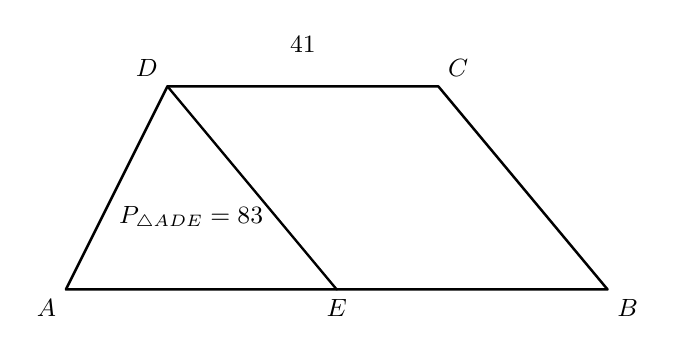
\begin{tikzpicture}[
  scale=0.86,
  line cap=round,
  line join=round,
  every node/.style={font=\small}
]
  \coordinate (A) at (0,0);
  \coordinate (B) at (8,0);
  \coordinate (D) at (1.5,3);
  \coordinate (C) at (5.5,3);

  % DE параллельна CB
  \coordinate (E) at (4,0);

  % Трапеция
  \draw[line width=0.9pt]
    (A)--(B)--(C)--(D)--cycle;

  % Прямая, параллельная боковой стороне
  \draw[line width=0.85pt] (D)--(E);

  % Меньшее основание
  \path (D)--(C)
    node[midway,above=3mm] {$41$};

  % Периметр отсечённого треугольника
  \node at (1.85,1.05)
    {$P_{\triangle ADE}=83$};

  % Подписи
  \node[below left]  at (A) {$A$};
  \node[below right] at (B) {$B$};
  \node[above right] at (C) {$C$};
  \node[above left]  at (D) {$D$};
  \node[below]       at (E) {$E$};
\end{tikzpicture}
\end{center}

\[
\boxed{\text{Ответ: }165}
\]


% =========================================================
% ВАРИАНТ 29
% =========================================================

\newpage

\section*{Вариант 29}

В треугольнике со сторонами \(8\) и \(4\) проведены высоты
к этим сторонам. Высота, проведённая к первой из этих сторон,
равна \(1\).
Чему равна высота, проведённая ко второй стороне?

\begin{center}
\begin{tikzpicture}[
  scale=0.82,
  line cap=round,
  line join=round,
  every node/.style={font=\small}
]
  % AB = 8, AC = 4, высота CH = 1
  \coordinate (A) at (0,0);
  \coordinate (B) at (8,0);
  \coordinate (C) at (3.873,1);

  % Основание высоты к AB
  \coordinate (H) at (3.873,0);

  % Основание высоты из B на продолжение AC
  \coordinate (D) at (7.5,1.936);

  % Треугольник
  \draw[line width=0.9pt]
    (A)--(B)--(C)--cycle;

  % Высота к стороне AB
  \draw[line width=0.8pt] (C)--(H);

  % Продолжение AC и высота из B
  \draw[dashed,line width=0.75pt] (C)--(D);
  \draw[line width=0.8pt] (B)--(D);

  % Прямые углы
  \pic[
    draw,
    line width=0.6pt,
    angle radius=3mm
  ] {right angle=C--H--B};

  \pic[
    draw,
    line width=0.6pt,
    angle radius=3mm
  ] {right angle=B--D--C};

  % Длины
  \path (A)--(B)
    node[midway,below=3mm] {$8$};

  \path (A)--(C)
    node[midway,above left] {$4$};

  \path (C)--(H)
    node[midway,right=2mm] {$1$};

  % Подписи
  \node[below left]  at (A) {$A$};
  \node[below right] at (B) {$B$};
  \node[above]       at (C) {$C$};
  \node[below]       at (H) {$H$};
  \node[above right] at (D) {$D$};
\end{tikzpicture}
\end{center}

\[
\boxed{\text{Ответ: }2}
\]


% =========================================================
% ВАРИАНТ 30
% =========================================================

\section*{Вариант 30}

Перпендикуляр, опущенный из вершины тупого угла
на большее основание равнобедренной трапеции,
делит его на части, имеющие длины \(10\) и \(9\).
Найдите среднюю линию этой трапеции.

\begin{center}
\begin{tikzpicture}[
  scale=0.95,
  line cap=round,
  line join=round,
  every node/.style={font=\small}
]
  % Отрезки основания изображены в пропорции 10 : 9
  \coordinate (A) at (0,0);
  \coordinate (B) at (7.6,0);
  \coordinate (E) at (4,0);

  \coordinate (D) at (3.6,2.6);
  \coordinate (C) at (4,2.6);

  % Равнобедренная трапеция
  \draw[line width=0.9pt]
    (A)--(B)--(C)--(D)--cycle;

  % Перпендикуляр
  \draw[line width=0.85pt] (C)--(E);

  \pic[
    draw,
    line width=0.65pt,
    angle radius=3.2mm
  ] {right angle=C--E--B};

  % Отметки равных боковых сторон
  \draw[line width=0.7pt]
    ($(A)!0.55!(D)+(-0.08,0.03)$)--
    ($(A)!0.55!(D)+(0.08,-0.03)$);

  \draw[line width=0.7pt]
    ($(B)!0.55!(C)+(-0.08,-0.03)$)--
    ($(B)!0.55!(C)+(0.08,0.03)$);

  % Длины частей основания
  \path (A)--(E)
    node[midway,below=3mm] {$10$};

  \path (E)--(B)
    node[midway,below=3mm] {$9$};

  % Подписи
  \node[below left]  at (A) {$A$};
  \node[below right] at (B) {$B$};
  \node[above right] at (C) {$C$};
  \node[above left]  at (D) {$D$};
  \node[below]       at (E) {$E$};
\end{tikzpicture}
\end{center}

\[
\boxed{\text{Ответ: }10}
\]

\end{document}